\section{Lunchapp - Proof of Concept}
\label{section:realisation:lunchapp}

\subsection{Beschreibung}
Die Idee der Lunchapp ist es, den Medienbruch zu den Offline-Mitarbeitern möglichst früh zu nehmen und eine App zu entwickeln, die kontinuierlich von den Mitarbeitern genutzt wird. Während der Nutzung wird der Mitarbeiter gefragt, ob er an einer Umfrage teilnehmen möchte, und kann dies direkt aus der App tun. Der Vorteil einer Lunchapp ist vor allem, dass es sich um unkritische Daten handelt. Um diesen Punkt zu verdeutlichen, wird eine andere Möglichkeit weiter beleuchtet: Der Dienstplan. Hierbei handelt es sich um datenschutzrechtlich sensible Daten, die keineswegs frei verfügbar gemacht werden dürfen. Dementsprechend wurde für eine prototypische Implementierung eine Lunchapp ausgewählt.
\subsection{Lastenheft}

\begin{itemize}
\item Es ist eine mobile Anwendung zu erstellen, die das Lunchmenü für die nächsten 5 Tage anzeigt. Dies beinhaltet den Namen, den Preis sowie die Allergene und Zusatzstoffe der einzelnen Menüs.
\item Zusätzlich sollen die Öffnungszeiten der Kantine angezeigt werden. 
\item Außerdem soll es möglich sein zwischen verschiedenen Kantinen zu wählen.
\item Wenn die Kantine geschlossen ist, soll diese Information anstelle der Öffnungszeiten und des Lunchmenüs angezeigt werden.
\item Des Weiteren soll die Umfragefunktionalität von PulseShift direkt innerhalb der Anwendung zur Verfügung stehen und kein Absprung nötig sein.
\item In der Anwendung sollen Banner angezeigt werden können, die den Nutzer zum Teilen der App oder der Teilnahme an einer Umfrage bewegen. Diese sollen in für den Nutzer als zufällig empfundenen Zeitabständen angezeigt werden.
\item Für die Umfragefunktionalität soll der Benutzer mindestens auf eine Gruppe von Personen eingegrenzt werden können.
\item Der Nutzer soll von der Anwendung aktiv über die Möglichkeit zur Umfrage, sowie Essensangebote informiert werden.
\item Das Design der Anwendung soll sich an den von PulseShift entwickelten und bereitgestellten Mockups orientieren.
\end{itemize}

\subsection{Pflichtenheft}

\begin{itemize}
\item Es wird eine \gls{pwa} erstellt, die auf verschiedenen Plattformen lauffähig ist. 
\item Diese ermöglicht das Anzeigen des Lunchs für die nächsten 5 Tage mit dem Namen, dem Preis sowie den Allergenen und Zusatzstoffen der einzelnen Menüs. 
\item Außerdem werden die Öffnungszeiten sowie eine mögliche Schließung der Kantine angezeigt.
\item Die Daten zum Lunchmenü und den Öffnungszeiten werden lokal und hart kodiert in einer JSON Datei gemockt. Eine Anbindung an einen Datenserver erfolgt nicht. 
\item Die Umfragefunktionalität, die von PulseShift entwickelt wurde, wird in die Anwendung hineingerendert werden. Das Anzeigen der Umfrage wird nicht selbst implementiert. 
\item Der Server für die Umfragefunktionalität wird austauschbar sein. Damit ist gemeint, dass die URL beliebig definierbar ist.
\item Die Benutzereingrenzung wird nach einer Absprache mit PulseShift über die konkrete gewünschte Ausprägung implementiert.
\item Die Detailansicht der Lunchmenüs wird dynamisch in die View der Übersicht des Lunchmenüs integriert.
\item Es wird eine Bannerfunktionalität bereitgestellt, die dynamisch ausgelöst werden soll. Diese weißt den Nutzer auf das Teilen der Anwendung, sowie die Möglichkeit zur Umfrage hin.
\item Für Android Geräte werden Pushbenachrichtigungen implementiert. Für iOS ist dies aufgrund der Realisierung als \gls{pwa} nicht möglich.
\item Die Anwendung wird lokal gecached, damit sie auch ohne Internetverbindung genutzt werden kann.
\end{itemize}

\subsection{EPK: Ablauf der Anwendung}

Die Nutzerinteraktion beginnt mit dem Öffnen der \gls{pwa}. Dabei gibt es wie in Abbildung \ref{fig:lunchepk} dargestellt drei verschiedene Möglichkeiten. Zum einen kann es sein, dass ausschließlich das Lunchmenü erscheint, mit dem der Benutzer interagieren kann. Zum anderen können aber auch zusätzlich entweder ein Umfragebanner oder ein Teilen-Banner angezeigt werden. Über das Umfrage-Banner kann der Anwender an der in die Applikation integrierte Umfrage teilnehmen. Das Teilen-Banner ermöglicht es ihm, die Lunchapp per Mail oder über soziale Netzwerke mit seinen Kollegen zu teilen.

\begin{figure}[H]
\centering
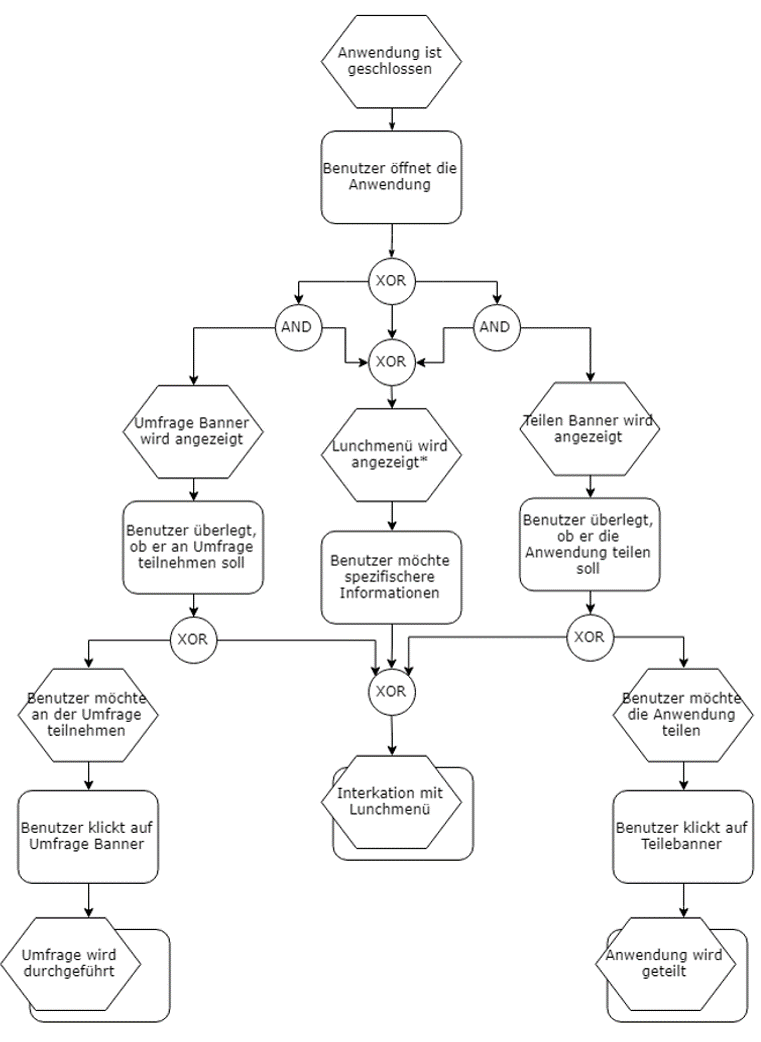
\includegraphics[width=0.8\textwidth]{images/lunchapp_epk}
\caption[EPK der Lunchapp]{EPK der Lunchapp}
\label{fig:lunchepk}
\end{figure}

Bezüglich der Interaktion des Nutzers mit dem Lunchmenü stehen ihm drei wesentliche Funktionalitäten zur Verfügung (siehe Abbildung \ref{fig:lunchepkdetail}). Er kann auf eine spezifische Speise klicken und sich Details, wie zum Beispiel enthaltene Zusatzstoffe ansehen. Außerdem kann er zwischen verschiedenen Kantinen, aber auch Wochentagen, wechseln.

\begin{figure}[H]
\centering
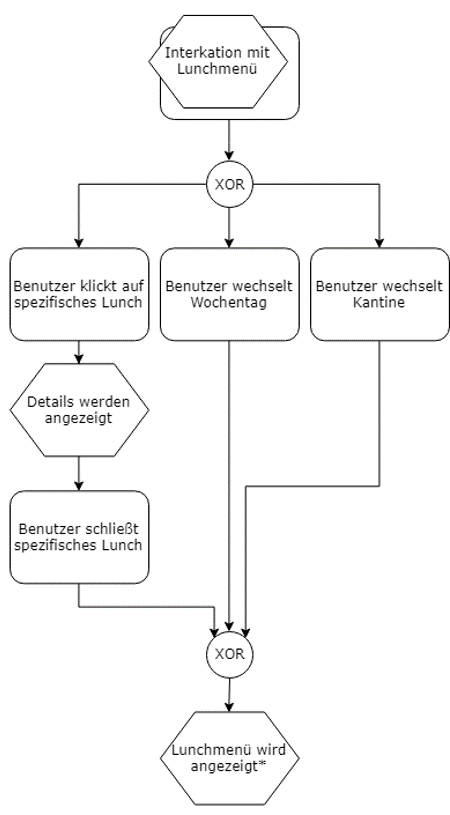
\includegraphics[width=0.5\textwidth]{images/lunchapp_epk_detail}
\caption[Interaktion mit dem Lunchmenü]{EPK der Lunchapp: Interaktion mit dem Lunchmenü}
\label{fig:lunchepkdetail}
\end{figure}

\subsection{Architektur}

Abbildung \ref{fig:laarchitecture} zeigt die grobe Architektur der Lunchapp. Die gesamte Anwendung ist auf einem Firebase-Server deployt. Die in der Firebase gespeicherten Daten sind mit dem Model der Vue.js Applikation synchronisiert und werden auf der LunchListView angezeigt. Der Controller übernimmt insbesondere das Routing zwischen LunchListView und SurveyView, zum Beispiel beim Klicken auf das Umfragebanner. In die SurveyView wird die Umfrage vom PulseShift-Server gerendert.   

\begin{figure}[H]
\centering
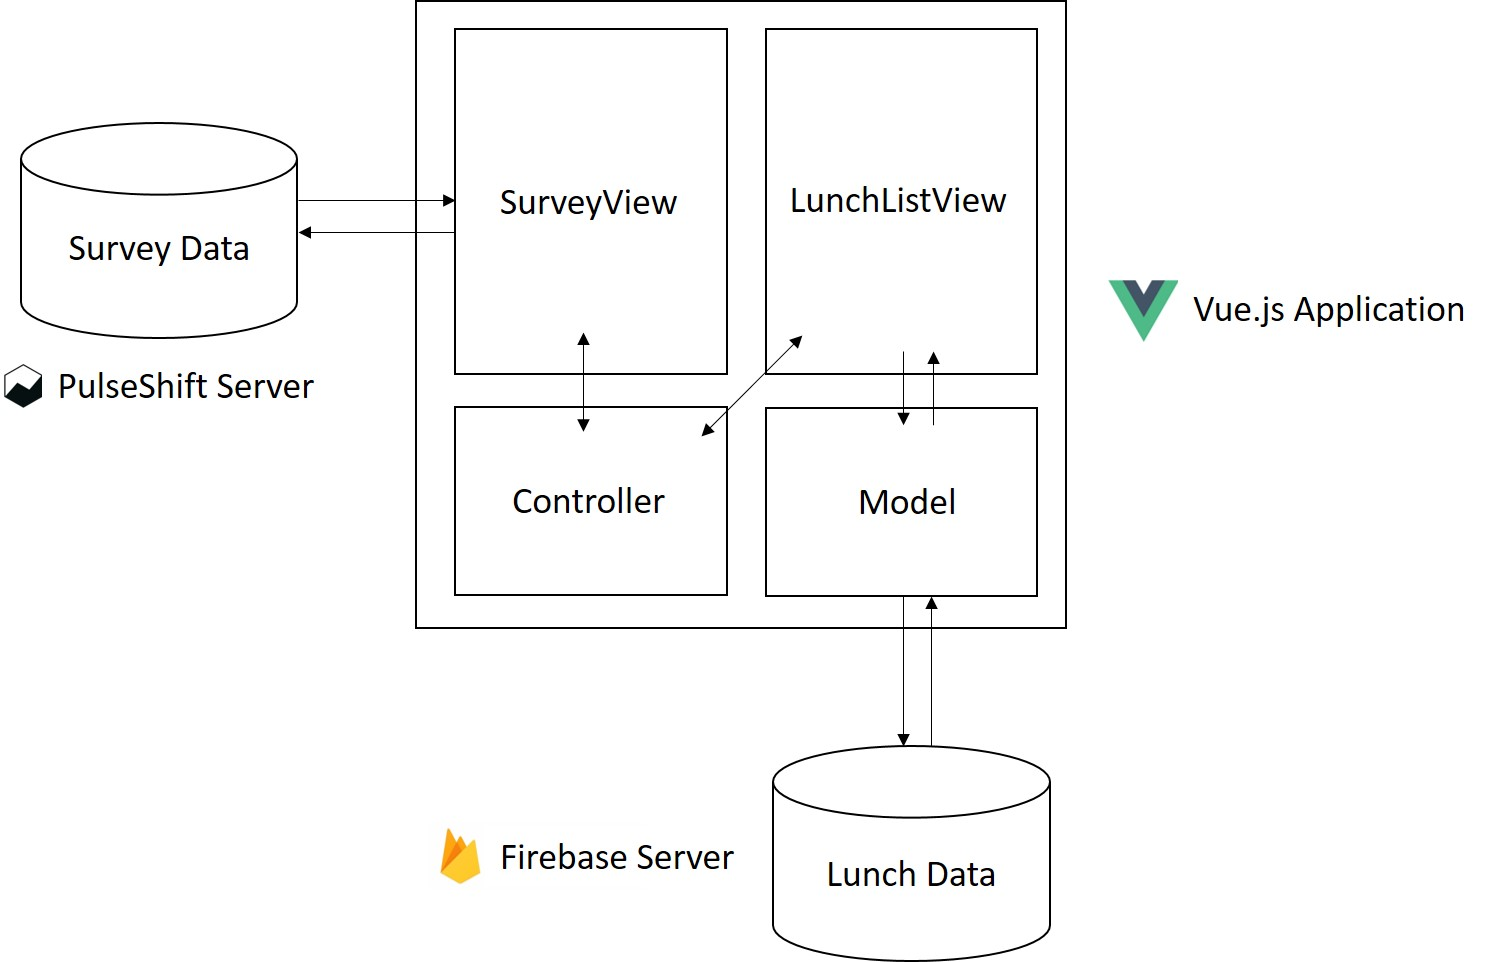
\includegraphics[width=0.9\textwidth]{images/lunchapp_architecture.jpg}
\caption[Architektur der Lunchapp]{Architektur der Lunchapp}
\label{fig:laarchitecture}
\end{figure}

\subsection{Komponenten}

Im Folgenden werden grundlegende architektonische Entscheidungen gelistet und jeweils begründet.

Zunächst wurde sich für eine \gls{pwa} entschieden, und gegen eine Umsetzung als hybride Applikation. Um diese Entscheidung ausreichend begründen zu können, werden beide Technologien kurz vorgestellt.

Eine hybride Applikation ist eine native App, die aber mit Web-Technologien umgesetzt wird. Dies bedeutet, dass die Web-App in einem nativen Container ausgeführt wird und auch über einige native Funktionen verfügen kann. Nachteilig wirkt sich diese Technologie vor allem bei der Performance und der User Experience aus. Nutzer berichten, dass sich die Applikation unecht anfühlt, und gerade bei größeren Datenmengen und anspruchsvollen Routinen langsam wird. Allerdings brauch der Anbieter die App zum größten Teil nur einmal entwickeln und kann sie mit wenig Anpassungen auf allen Plattformen anbieten. Auch wenn diese Technologie vielversprechend sein mag, ist eine \gls{pwa} für den vorliegenden Anwendungsfall die bessere Wahl.

Eine \gls{pwa} ist eine Web-Applikation, die sich der Nutzer über das Speichern auf dem Home-Screen lokal abspeichern kann. Durch sogenannte Service-Worker können zudem eingeschränkt native Funktionalitäten genutzt werden, zum Beispiel das Senden von Push-Benachrichtigungen, sowie das Cachen von Daten, und die daraus resultierende Offline-Nutzbarkeit. Für den vorliegenden Use-Case sind eben genau diese beiden Funktionalitäten ausreichend. Weiterhin wird die App über einen beliebigen Browser installiert, und muss nicht über den jeweiligen App-Store heruntergeladen werden. Das erhöht die Adaption der App und erleichtert den Unternehmen die Verteilung, da die für native Applikation notwendige Infrastruktur nicht vorhanden sein muss.

Da eine \gls{pwa} eine Web-Applikation ist, sind entsprechende Frameworks auszuwählen. In Anbetracht der begrenzten Zeit und mangelnden personellen Ressourcen wurde Vue.js als Framework gewählt. Alternativen wie React.js und Angular.js erscheinen zwar mächtiger, sind aber auch zeitaufwendiger in der Einarbeitung. Zudem lässt sich der begrenzte Umfang der App auch problemlos mit Vue.js realisieren und im Anschluss warten.

Um ein möglichst übersichtliches und modernes Design zu erhalten, wird Material Design eingesetzt. Gegenüber Alternativen wie beispielsweise Bootstrap hat es den Vorteil, dass es für mobile Applikationen subjektiv bewertet ein ansprechendes Design bietet. Um eine reibungslose Nutzung von Material Design Komponenten in Vue.js zu ermögichen, wird auf Vuetify zurückgegriffen, welches Material Design in Vue.js implementiert.

\subsubsection{Banner}

Die Banner, die sich direkt über dem eigentlichen Lunchmenü anzeigen lassen, stellen eine zentrale Komponente der Applikation dar. Durch das Umfragebanner (siehe Abbildung \ref{fig:banners}, links) wird der Mitarbeiter auf eine Unternehmensumfrage aufmerksam gemacht und kann mit einem Klick auf $"$Teilnehmen$"$ auf die Survey-View gelangen, auf der er die vom PulseShift-Server geladenen Fragen beantworten kann.

\begin{figure}[H]
\centering
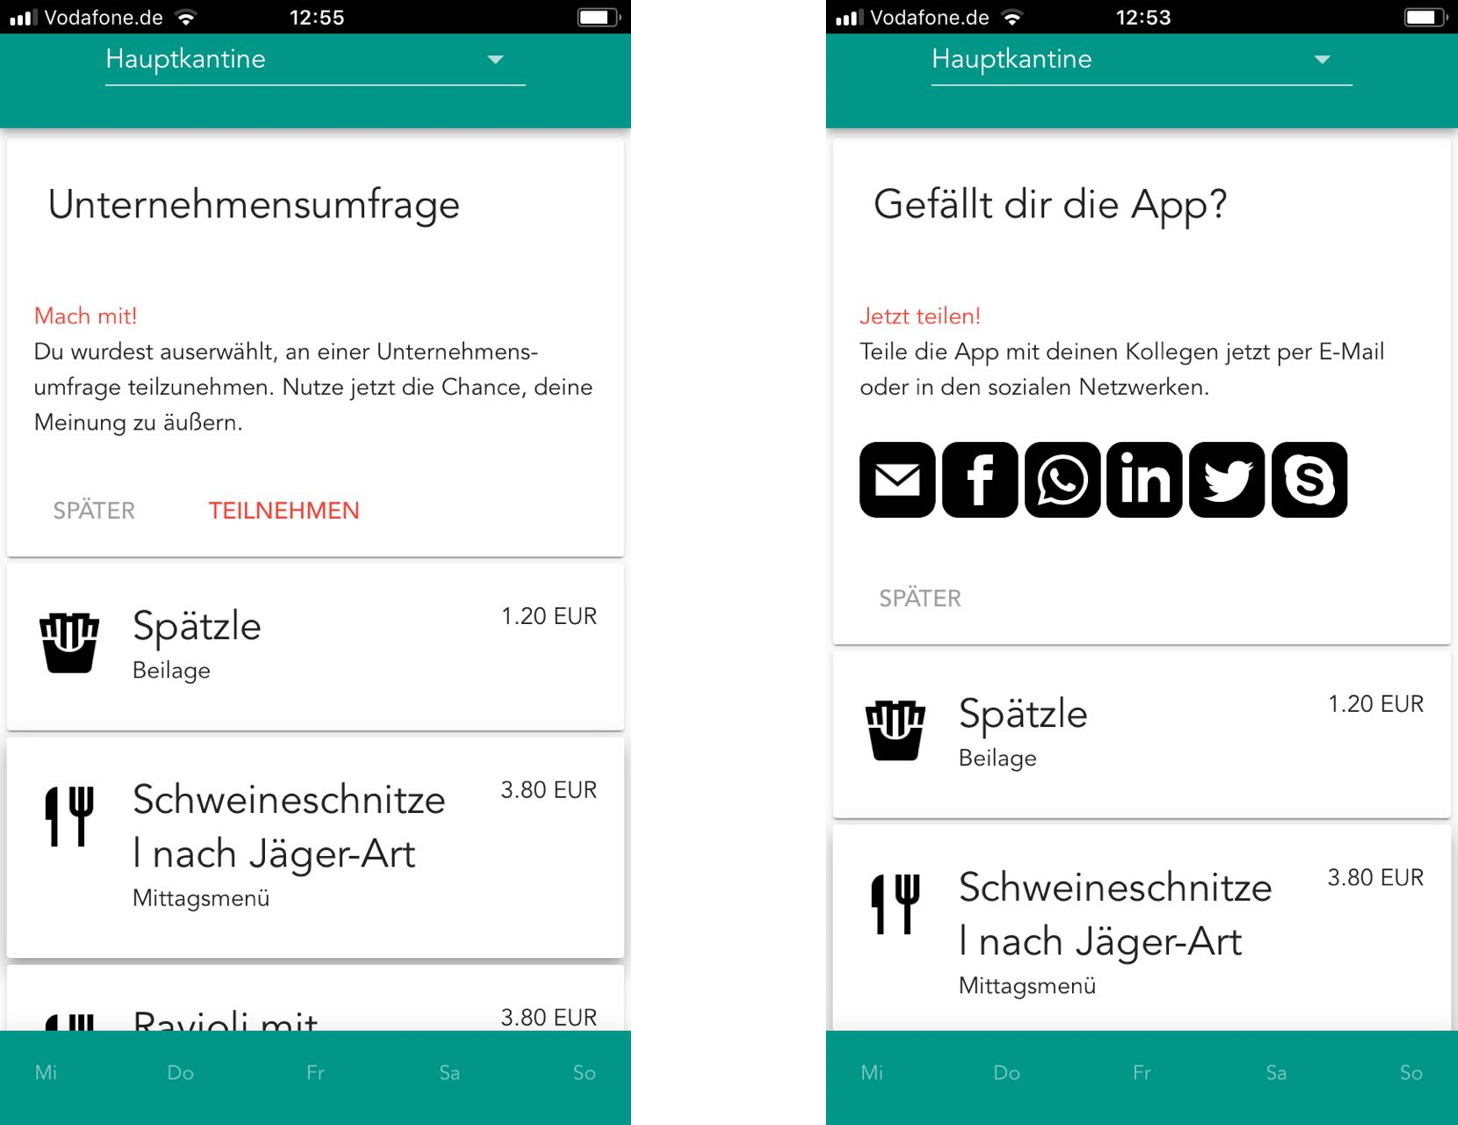
\includegraphics[width=0.9\textwidth]{images/banners}
\caption[Umfrage- und Teilen-Banner]{Umfrage- und Teilen-Banner}
\label{fig:banners}
\end{figure}

Das Teilen-Banner (siehe Abbildung \ref{fig:banners}, rechts) ermöglicht es dem Nutzer, die Applikation mit seinen Kollegen zu teilen. Neben dem Versenden einer E-Mail stehen ihm dabei die sozialen Netzwerke Facebook, LinkedIn und Twitter, sowie die Messenger Skype und WhatsApp zur Verfügung.

Die Banner werden dynamisch mithilfe von Conditional Rendering eingebunden und derzeit zufällig beim Öffnen des Lunchmenüs getriggert, wobei das Umfragebanner nur angezeigt wird, wenn der Nutzer online ist. Für den produktiven Einsatz müsste jedoch ein externer Trigger-Mechanismus implementiert werden, der es PulseShift ermöglicht die Umfragen beliebig zu schalten.



\subsubsection{Push Notification}
Die Push Notification soll ermöglichen, dass der Benutzer der \gls{pwa} Benachrichtigungen auf sein beliebiges Endgerät erhält. So kann es ermöglicht werden, die Aufmerksamkeit des Nutzers auf die App und somit auch die Umfrage zu lenken. 

Vorab muss jedoch geprüft werden, ob das Endgerät oder auch der benutze Browser die Push Notifications unterstützen. 

\begin{itemize}
\item Zunächst wird geprüft, ob der Services Worker bereit ist. 
\item Danach wird geprüft, ob dieser Services Worker in der Lage ist Push Notifications zu verarbeiten.
\item Daraufhin wird geprüft, ob das geöffnete Fenster die Push Notifications überhaupt unterstützt.
\item Im nächsten Schritt wird geprüft, ob die Push Notifications schon abgelehnt wurden. Bei diesem Schritt kann darauf hin entweder erneut gefragt werden oder einfach ohne Push Notifiactions die App bedient werden.
\end{itemize} 

Wird die Seite aufgerufen und die Push Notification sind technisch möglich wird der Benutzer mit einem Pop-Up darauf hingewiesen, dass er die Möglichkeit hat diese zu erhalten. 

Hat der Benutzer sich dazu entschlossen die Push Notifications einzuschalten, können nun von außen Nachrichten an den Benutzer gesendet werden. Dazu wird die Entwicklungs-Plattform Firesbase genutzt. Mit Hilfe von Firebase können nun die Benachrichtigungen in bestimmten zeitlichen Abständen gesendet werden.

\subsection{Anforderungserfüllung}
Die im Lasten- und Pflichtenheft beschriebenen Anforderungen konnten weitestgehend erfüllt werden. Im Folgenden wird das finale Produkt mit dem Pflichtenheft verglichen. 
\begin{figure}[H]
\centering
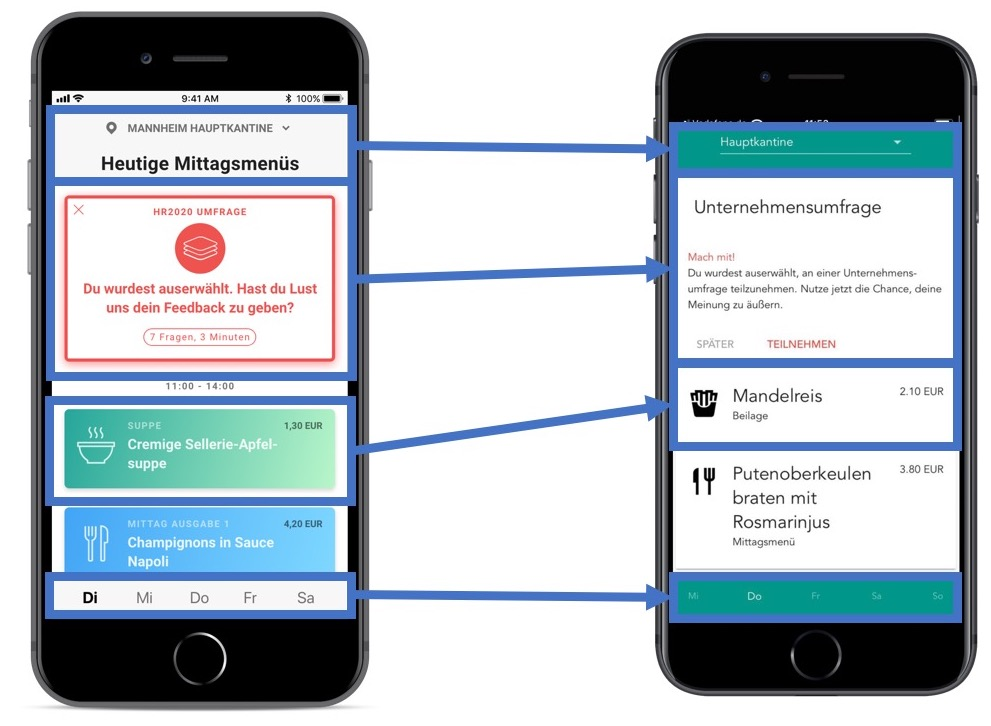
\includegraphics[width=0.7\textwidth]{images/docs-comparison}
\caption[Vergleich des Mockups mit dem finalem Produkt]{Vergleich des Mockups mit dem finalem Produkt}
\label{fig:mockup-comparison}
\end{figure}

Während der Beschreibung wird auf\vref{fig:mockup-comparison} Bezug genommen, welches das vom Unternehmen bereitgestellte Mockup mit dem finalen Produkt vergleicht.

\begin{itemize}
\item Die Umsetzung als \gls{pwa} wurde erfolgreich durchgeführt. Das Design der finalen App kommt dementsprechend nur vom Aufbau, nicht aber vom Aussehen an das Mockup heran. Durch die Umsetzung als Web-Applikationen mussten entsprechende Änderungen vorgenommen werden, was aber durch die Vorgabe, eine\gls{pwa} zu erstellen durchaus gewollt ist.
\item Wie in\vref{fig:mockup-comparison} zu sehen, zeigt die App das Menü für die nächsten fünf Tage und verschiedenen Kantinen an. Weiterhin wird der Nutzer, wie vorausgesetzt über Preis und Zusatzstoffe, sowie Allergene informiert. Letzteres wird sichtbar, wenn der Nutzer auf ein Menü drückt.
\item Die Öffnungszeiten, sowie eine mögliche Schließung der Kantine wird ebenfalls angezeigt. Im Falle einer Schließung wir dem Nutzer die entsprechende Information gegeben, der Tag ist aber trotzdem auswählbar.
\item Umfangreiche Mockdaten wurden erfolgreich erstellt und sind lokal in der App verfügbar. Ein Backendservice wurde nicht gebaut, eine Integration mit beispielsweise Google Firebase ist durch die Struktur der Applikation allerdings kein großer Aufwand mehr.
\item Die Umfragefunktionalität von PulseShift wird durch ein iFrame in die App gerendert. Allerdings hat die produktive Version des Servers noch Restriktionen, die eine Einbindung nicht erlauben. Währenddessen diese entfernt werden, wird auf eine lokale Version zurückgegriffen.
\item Die Umfragefunktionalität ist innerhalb weniger Sekunden austauschbar.
\item Eine Benutzereingrenzung wurde nicht konkret in die Applikation implementiert, allerdings lässt sich dies durch die Realisation als Web-Applikation über beispielsweise QR-Codes im produktiven Einsatz einfach umsetzen.
\item Die Detailansicht der einzelnen Menüs ist wie vorgesehen dynamisch in der View implementiert.
\item Die entsprechende Bannerfunktionalität wurde erfolgreich implementiert. Der Nutzer bekommt für die Demo-Version die Banner mit einer gewissen Wahrscheinlichkeit beim Öffnen der Applikation angezeigt.
\item Für Google-Software wurden Pushbenachrichtigungen erfolgreich implementiert. Durch Restriktionen seitens Apple kann dies für entsprechende Geräte allerdings zum heutigen Zeitpunkt nicht realisiert werden. Jedoch ist Apple committed, dies in der Zukunft zu ermöglichen.
\item Die Anwendung wird wie vorgesehen lokal gecached und kann auf allen Plattformen, somit auch Offline, vollständig genutzt werden.
\end{itemize}